\chapter{Model konceptualny i fizyczny baz danych}

\section{Model konceptualny}

\begin{figure} [H]
	\centering
	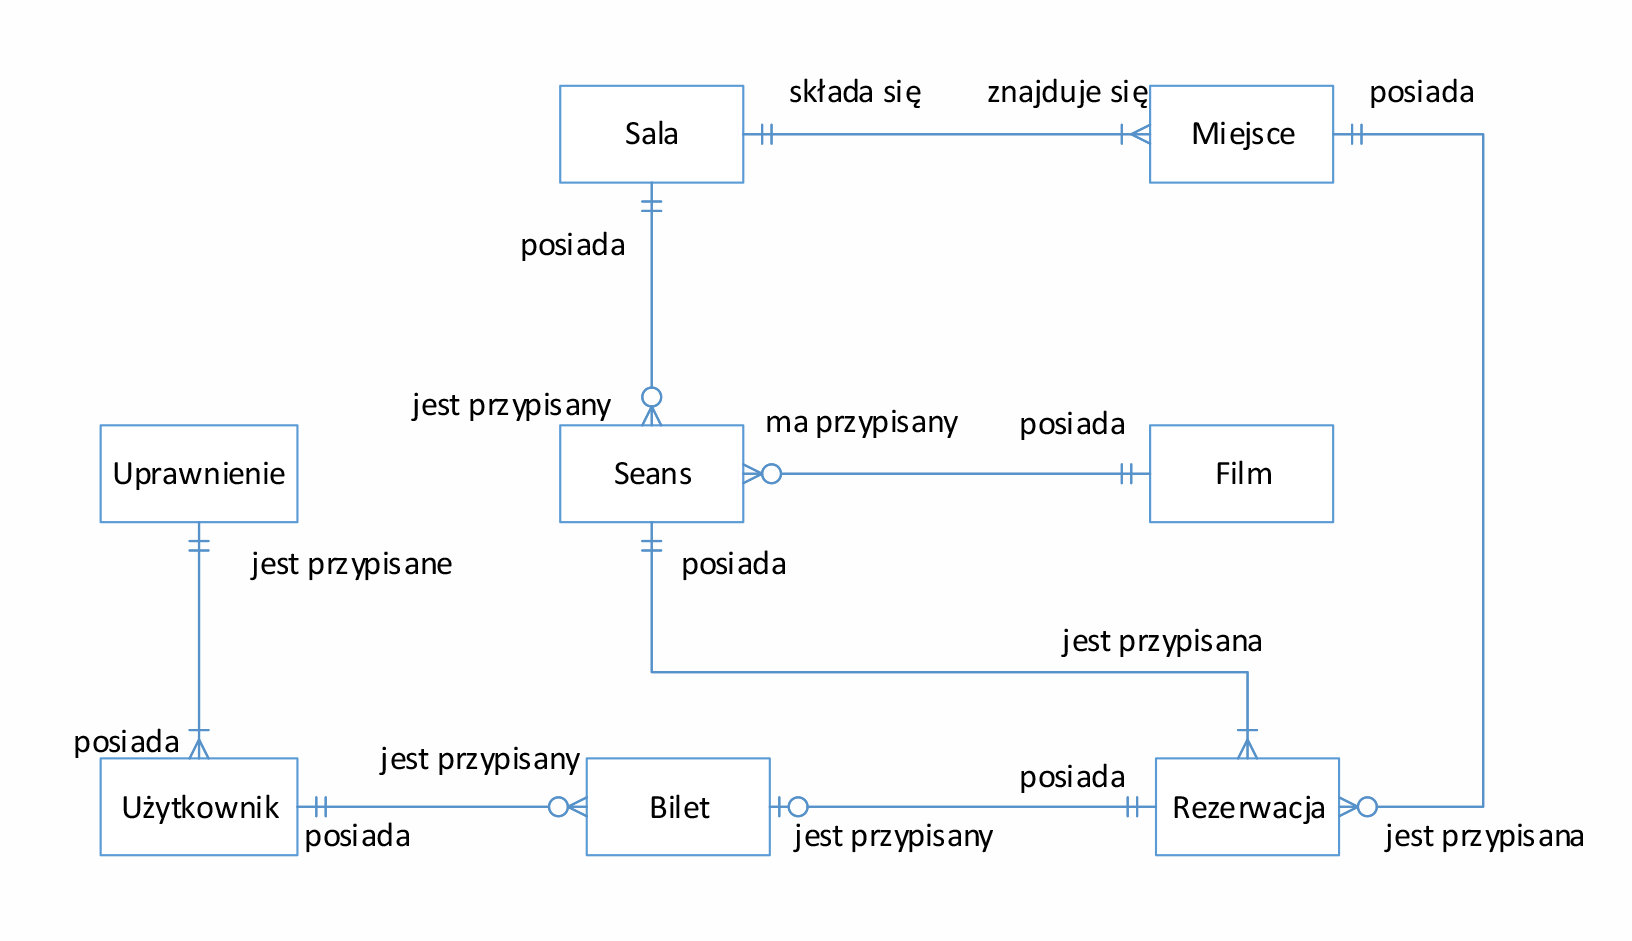
\includegraphics[width=1\linewidth]{rozdzial03/model_konceptualny.png}
	\caption{Model konceptualny węzła rozproszonej bazy danych wykonany w programie Microsoft Visio}
	\label{fig:model_koncepcyjny}
\end{figure}

W bazie danych dominują relacje typu jeden do wielu. Na każdej sali może odbywać się wiele seansów, natomiast każdy seans posiada tylko jeden film i jedną salę. Każde miejsce również ma przypisaną jedną konkretną salę. Na jedno miejsce może przypadać wiele rezerwacji, w zależności od seansu. Również każdy użytkownik może mieć wiele kupionych biletów lub nie mieć ich wcale. Oraz istnieje wielu użytkowników o tych samych uprawnieniach. Jedyną relacją, która nie jest jeden do wielu, to powiązanie między tabelą \textit{Bilety} i \textit{Rezerwacje}. Na każdą rezerwację może być maksymalnie jeden bilet, który odpowiada jednej rezerwacji, rozumianej tutaj jako miejsce na konkretny seans, które może być zajęte lub też nie.


\section{Model fizyczny}

\begin{figure} [H]
	\centering
	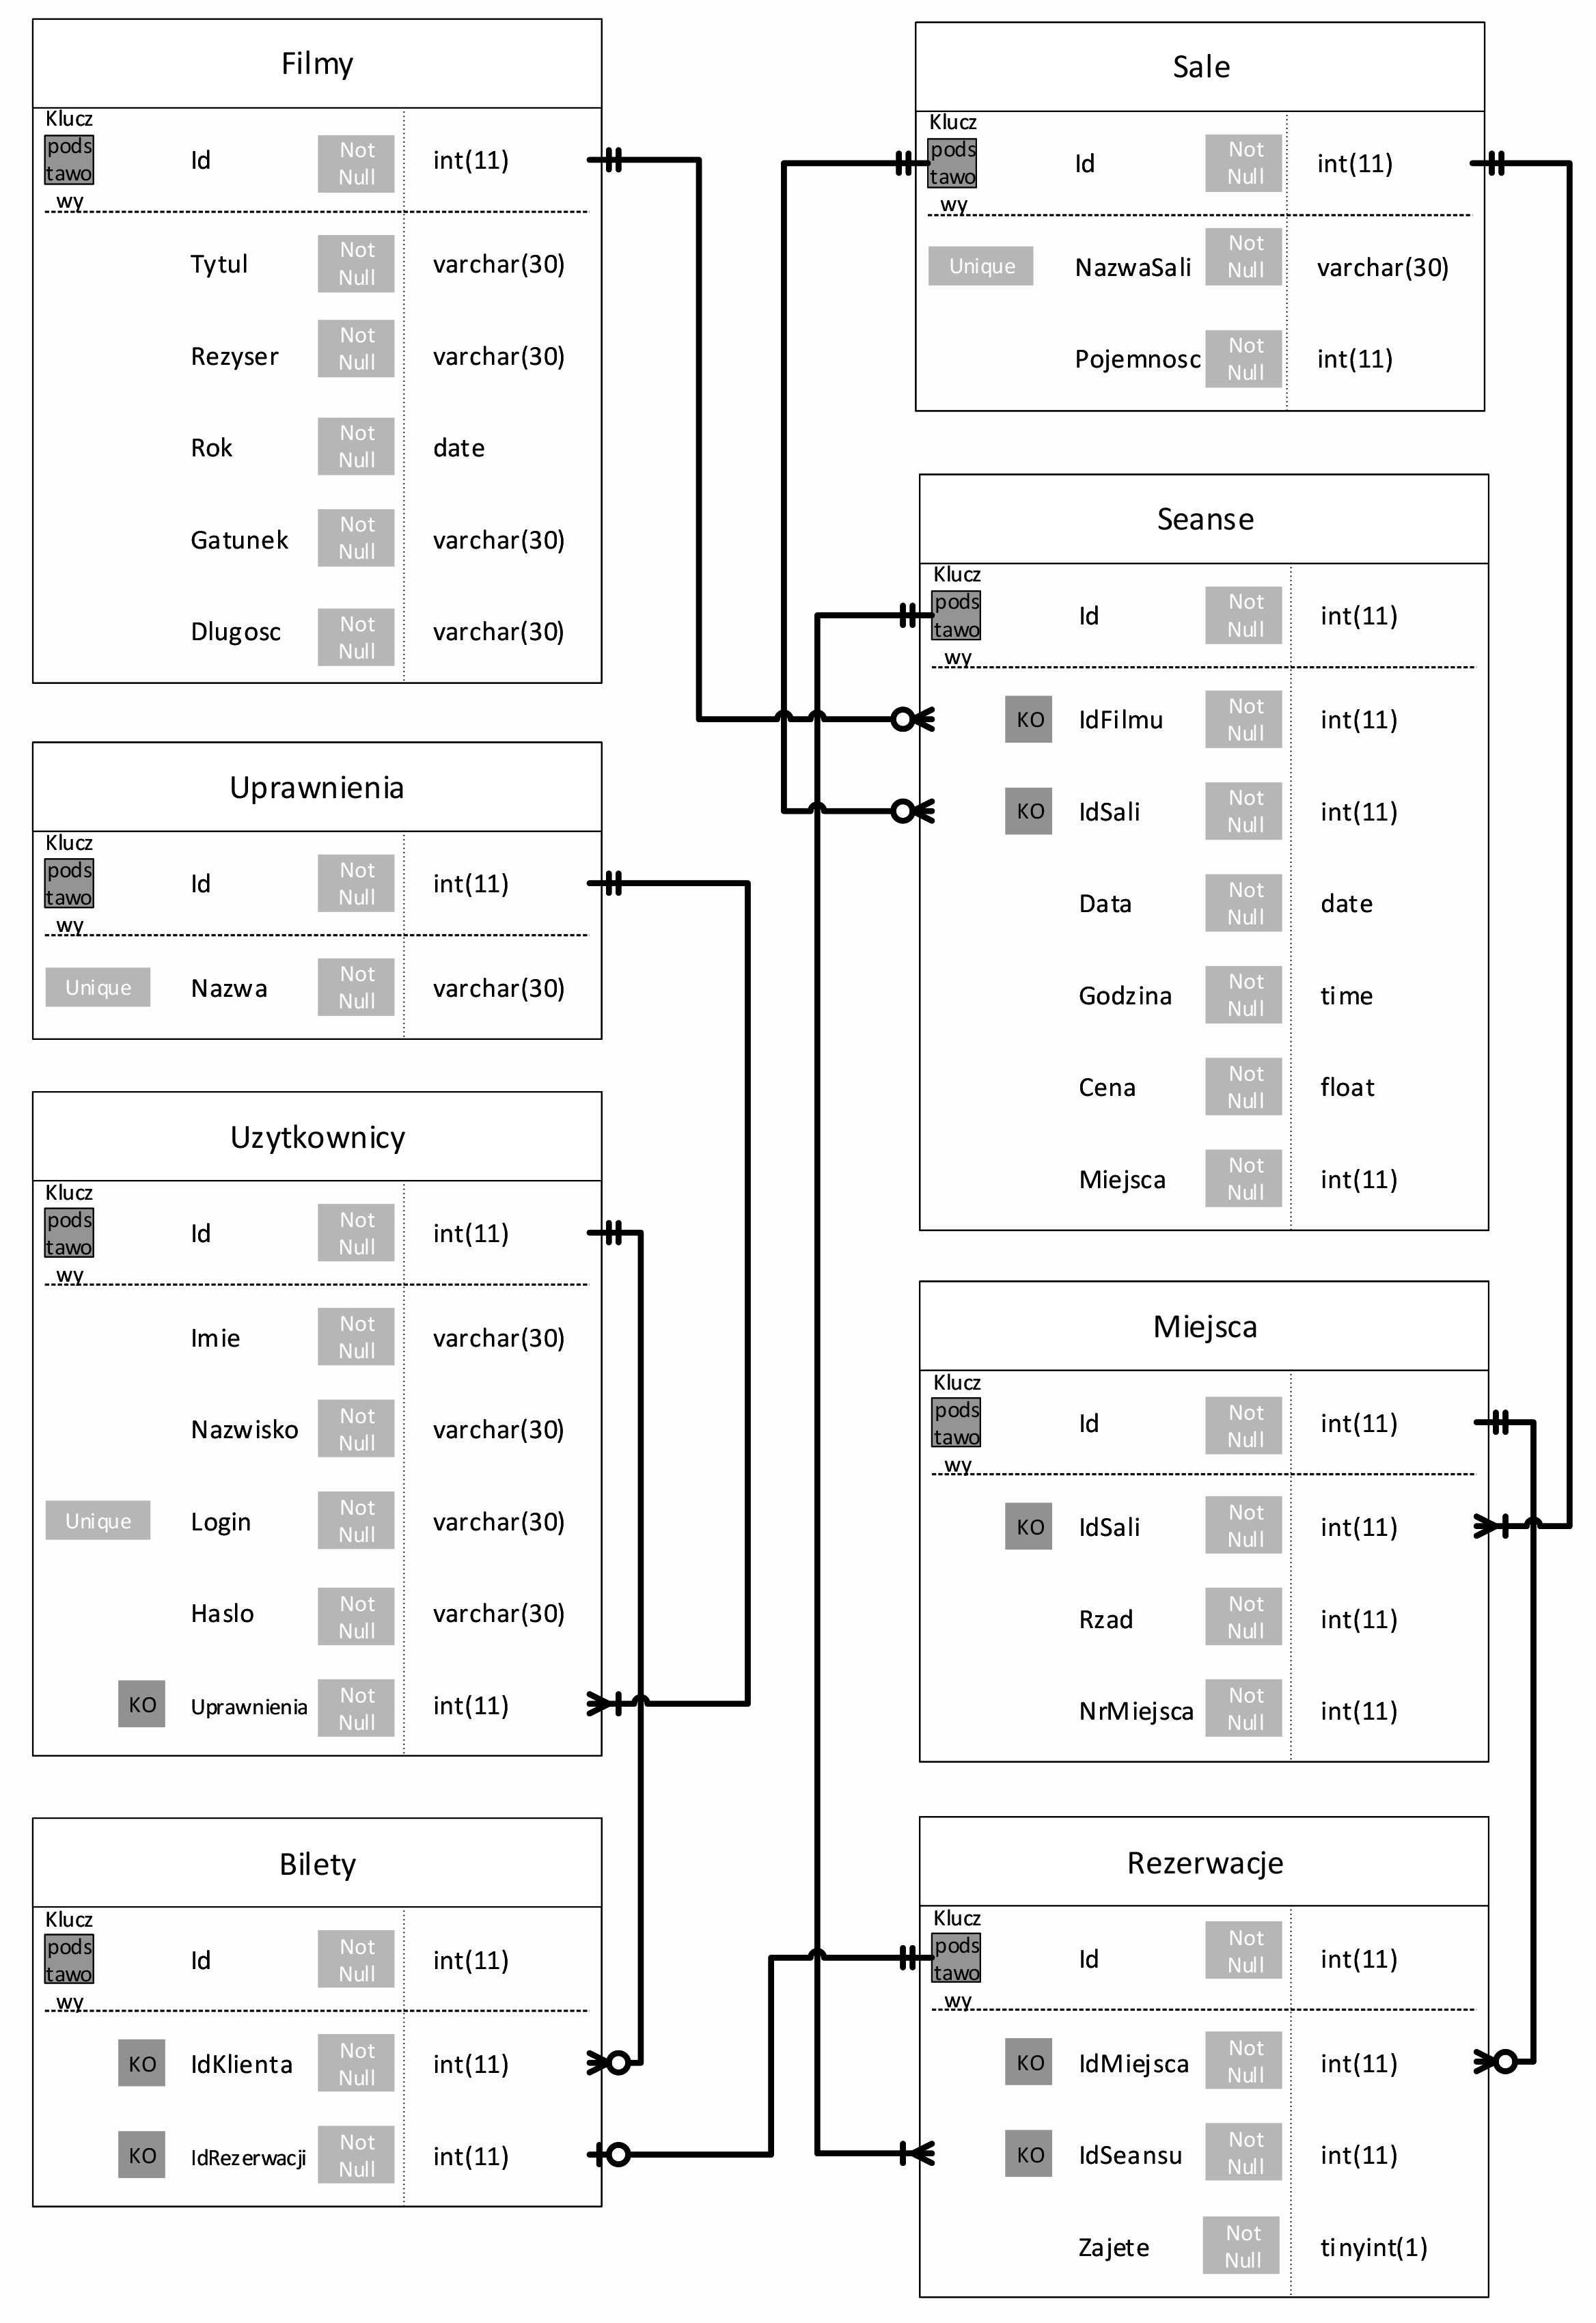
\includegraphics[width=0.95\linewidth]{rozdzial03/model_fizyczny.png}
	\caption{Model fizyczny węzła rozproszonej bazy danych wykonany w programie Microsoft Visio}
	\label{fig:model_fizyczny}
\end{figure}

\textbf{Tabele:}
\begin{itemize}
	\item \textit{Filmy} - przechowuje najważniejsze informacje o filmach, takie jak ich tytuł, nazwiska reżyserów, daty premiery, gatunek oraz czas trwania, żadna z tych wartości nie może pozostać pusta;
	\item \textit{Sale}	- jedynymi potrzebnymi w projekcie parametrami charakteryzującymi sale są jej unikalna nazwa i pojemność ukazująca liczbę dostępnych miejsc siedzących;
	\item \textit{Seanse} - każdy seans ma przypisany film oraz salę. Dodatkowo przechowuje takie informacje jak data i godzina wyświetlenia seansu, cenę oraz pozostałą liczbę wolnych miejsc;
	\item \textit{Miejsca} - w tej tabeli przechowywane są wszystkie miejsca siedzące dostępne w kinie. Każde miejsce znajduje się w swojej określonej sali. Każde miejsce dodatkowo ma też numer i rząd w którym się znajduje na sali;
	\item \textit{Rezerwacje} - jest to spis wszystkich miejsc na wszystkie dostępne seanse. Dodatkowo przechowywana jest wartość zero-jedynkowa odpowiadająca za stan czy miejsce jest już zajęte;
	\item \textit{Uprawnienia} - w projekcie przewidziane są uprawniania dwojakiego rodzaju: uprawniania administratora i użytkownika. Informacja ta ma kluczowe znaczenie podczas logowania do systemu i wyświetlania w nim dostępnych funkcjonalności;
	\item \textit{Użytkownicy} - każdy użytkownik jest zobligowany podczas procesu rejestracji do podania takich informacji o sobie jak imię i nazwisko, oraz podania hasła i unikalnego loginu przez który będzie się logował i to właśnie te dane są przechowywane w tej tabeli. Dodatkowo również do każdego użytkownika dodawane są jego uprawnienia: administratora lub zwykłego użytkownika;
	\item \textit{Bilety} - każdy bilet jest przypisany do konkretnego użytkownika i do konkretnego rekordu z tabeli \textit{Rezerwacje}.
\end{itemize}